\documentclass[onecolumn, draftclsnofoot,10pt, compsoc]{IEEEtran}
\hbadness=1000 % suppress warnings
\usepackage{graphicx}
\usepackage{url}
\usepackage{setspace}
\usepackage{hyperref}
\usepackage{listings}
\usepackage{cite}
\usepackage{geometry}
\usepackage{caption}

\geometry{textheight=9.5in, textwidth=7in}

% 1. Fill in these details
\def \CapstoneTeamName{			}
\def \CapstoneTeamNumber{		69}
\def \GroupMemberOne{			Kin-Ho Lam}
\def \GroupMemberTwo{			Lucien Armand Tamdja Tamno}
\def \CapstoneProjectName{		Depth Sensing using Computer Vision and Lydar}
\def \CapstoneSponsorCompany{	Oregon State University}
\def \CapstoneSponsorPerson{	D. Kevin McGrath}


% 2. Uncomment the appropriate line below so that the document type works
\def \DocType{		%Problem Statement
	%Requirements Document
	%Technology Review
	%Design Document
	Winter Midterm Progress Report
}

\newcommand{\NameSigPair}[1]{\par
	\makebox[2.75in][r]{#1} \hfil 	\makebox[3.25in]{\makebox[2.25in]{\hrulefill} \hfill		\makebox[.75in]{\hrulefill}}
	\par\vspace{-12pt} \textit{\tiny\noindent
		\makebox[2.75in]{} \hfil		\makebox[3.25in]{\makebox[2.25in][r]{Signature} \hfill	\makebox[.75in][r]{Date}}}}
% 3. If the document is not to be signed, uncomment the RENEWcommand below
\renewcommand{\NameSigPair}[1]{#1}

%%%%%%%%%%%%%%%%%%%%%%%%%%%%%%%%%%%%%%%
\graphicspath{{images/}}
\begin{document}
	\begin{titlepage}
		\pagenumbering{gobble}
		\begin{singlespace}
			\centering
			
\includegraphics[height=4cm,natwidth=345,natheight=435]{images/osu_logo.png}
			\hfill 
			% 4. If you have a logo, use this includegraphics command to put it on the coversheet.
			%\includegraphics[height=4cm]{CompanyLogo}   
			\par\vspace{.2in}
			\centering
			\scshape{
				\huge Senior Design Capstone \DocType \par
				{\large\today}\par
				\vspace{.5in}
				\textbf{\Huge\CapstoneProjectName}\par
				\vfill
				{\large Prepared for}\par
				\Huge \CapstoneSponsorCompany\par
				\vspace{5pt}
				{\Large\NameSigPair{\CapstoneSponsorPerson}\par}
				{\large Prepared by }\par
				Group\CapstoneTeamNumber\par
				% 5. comment out the line below this one if you do not wish to name your team
				\CapstoneTeamName\par 
				\vspace{5pt}
				{\large
					\NameSigPair{\GroupMemberOne}\par
					\NameSigPair{\GroupMemberTwo}\par
				}
				\vspace{20pt}
			}
			\begin{abstract}  
 				Depth Sensing with Computer Vision and LIDAR proposes combining computer vision and LIDAR to create a reliable depth sensor.
				This document details its project member’s progress toward a final design, and future milestones.
			\end{abstract}     
		\end{singlespace}
	\end{titlepage}
\section{Table of Contents}
\tableofcontents
\bibliographystyle{IEEEtran}
\bibliography{ref}
\clearpage

\begin{singlespace}
	\section{Definitions}

	\section{Project Purpose}
		Commercial infrared-based depth sensors such as the model used in Microsoft’s Kinect can quickly calculate distances in indoor scenarios.
		However, IR depth sensors can be confused by other infrared emitters such as other IR depth sensors or natural sunlight.
		For these reasons, IR depth sensors cannot be used in self-driving cars, outdoor robots, or any any device that requires high accuracy and reliable distance calculation.

		Depth Sensing with Computer Vision and LIDAR proposes combining the power of computer vision with the reliability of LIDAR technology.
		LIDAR uses a pulsing laser to measure relative distance.
		The LIDAR unit we're going to be using is called the RpLIDAR A1.
		We'll be combining this with a high-end logitech brio webcam.

	\section{Current State}

	\subsection{Kin-Ho Lam}
		\subsubsection{Proposed Design}
			The Logitech Brio webcam provides two-dimensional image but lacks depth perception.
			The RPLIDAR A1 LIDAR provides accurate depth measurement in a horizontal dimension but lacks vertical depth sensing.
			Combining the functionality of both devices to get accurate three-dimensional depth sensing presents a unique engineering challenge.
			This project proposes bridging the utility of both devices by securing them in stationary positions, then using software to combine their outputs.
			This involves using the RPLIDAR’s library to get depth sensing information, and using computer vision to recognize objects.
			
			\begin{figure}[h!]
				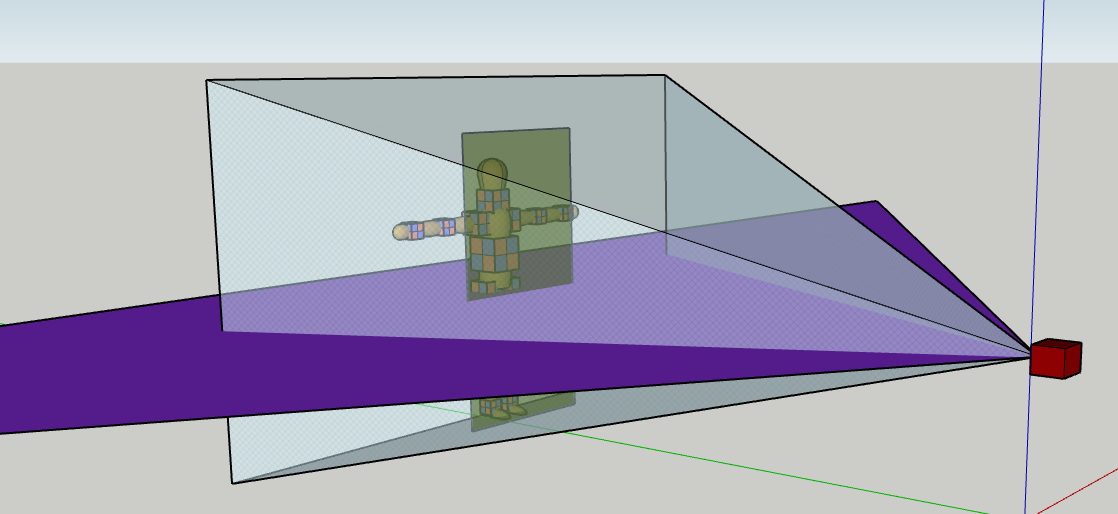
\includegraphics[scale=0.5, width=\textwidth]{different_dimensions.PNG}
				\label{dimensions}
				\captionof{figure}{Visualizing different dimensions measured by RPLIDAR and Brio Webcam.}
			\end{figure}

			In \ref{dimensions}, the red cube represents the Logitech Brio webcam and RPLIDAR device secured in stationary positions.
			The flat purple triangle represents the RPLIDAR’s horizontal range detection.
			The transparent green rectangle in front of the person represents the computer vision model recognizing that there is a person in-front of the sensor.
			The transparent teal pyramid represents the Brio webcam’s field-of-view.
			
			\begin{figure}[h!]
				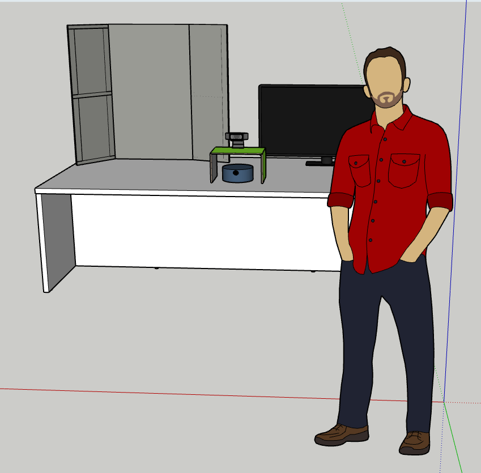
\includegraphics[scale=0.55]{expo.PNG}
				\label{fig:expo}
				\captionof{figure}{Expo/final design concept}
			\end{figure}

			\ref{fig:expo} illustrates the project’s final expo design.
			This render depicts the Brio webcam and RPLIDAR A1 in fixed positions.
			The software shall be capable of displaying the video output of the webcam with object distance information overlaid.
			The Brio webcam serves to provide subject identification and a point of reference in the vertical axis.
			The RPLIDAR A1 serves to provide distance measurement in the horizontal plane.
			As illustrated in \ref{fig:dimensions}, the horizontal range of the RPLIDAR A1 extends beyond the Brio webcam’s field of view.
			This requires software adjustments such that the RPLIDAR A1’s data is restricted to only collecting data within the camera’s FOV.
			Fixing both devices in stationary positions simplifies this task.
			Once relevant distance information can be parsed, the software shall then use computer vision to recognize contiguous objects such as people.
			If a person is identified and the RPLIDAR A1 detects an object is within the camera’s field of view, the software shall overlay distance 

			\begin{figure}[h!]
				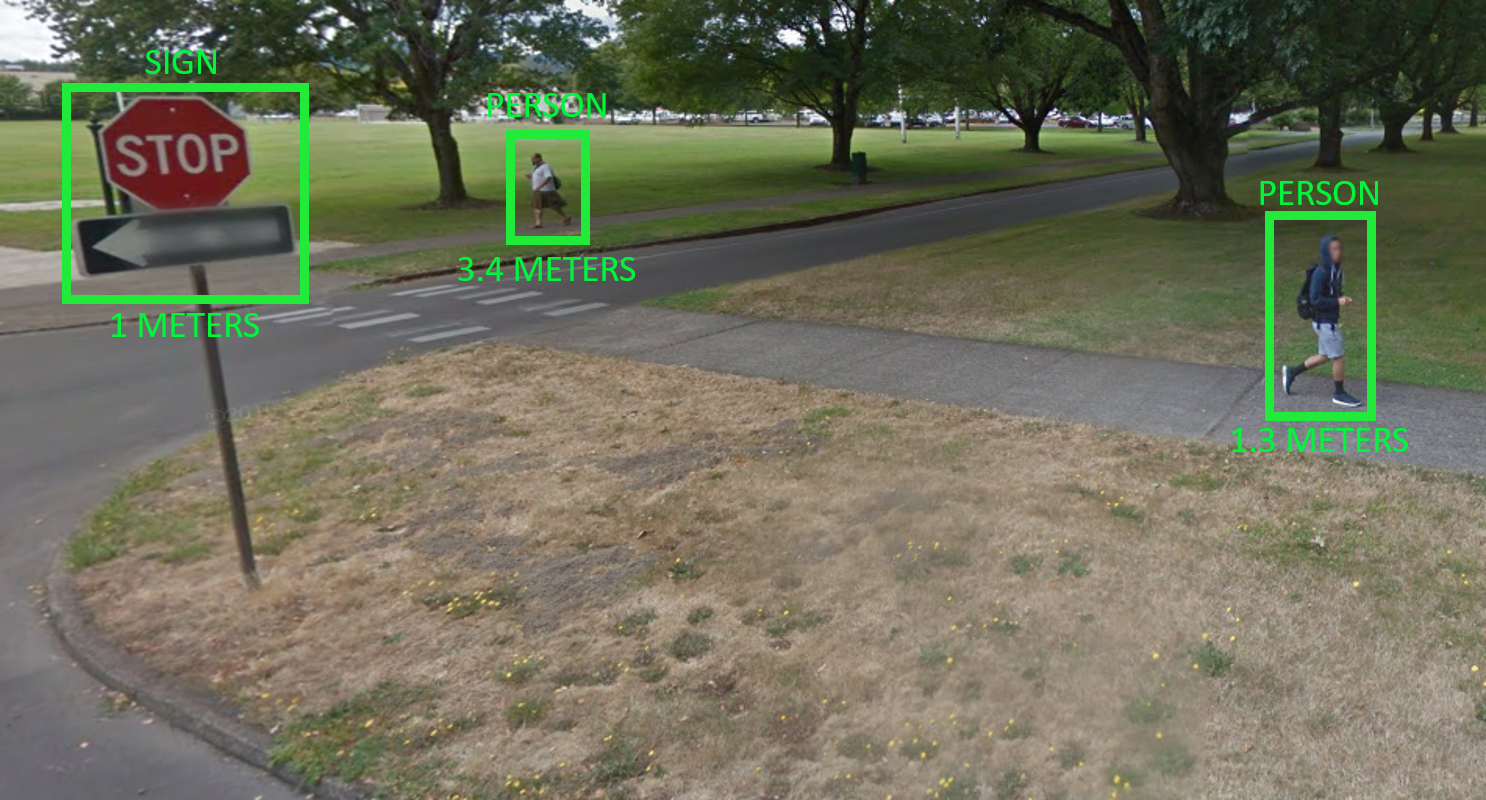
\includegraphics[scale=0.5, width=\textwidth]{overlay_design.png}
				\label{fig:overlay}
				\captionof{figure}{Distance overlay concept}
			\end{figure}

		\subsubsection{Computer Vision}
			\ref{fig:overlay} illustrates my current progress towards creating an accurate computer vision model.
			I am modifying a pre-trained SVM to recognize faces.
			The SVM can recognize faces in various lighting conditions even if the subject is wearing hats or glasses.
			This algorithm is not completely reliable or accurate, if the subject turns their face away from the camera or is looking off-center, the model will fail to recognize their face.
			This program is written in Python 3 and uses OpenCV 3.4.0.

		\subsubsection{Future Milestones}
			I hope to expand the SVM’s capabilities to recognize full or half bodies.
			I am exploring open-source algorithms to perform this task, and I am confident recognizing full or half bodies is possible.
			After my colleague Lucian completes his research into extracting depth sensing information from the RPLIDAR, I shall assist him in calibrating the software to only perform depth measurements within the webcam’s field of view.


	\section{Lucien Armand Tamdja Tamno}
\end{singlespace}
\end{document}
